\documentclass[a4, oneside, headings=normal]{scrartcl}

\usepackage{../latex/mystyle}
\addbibresource{tache8.bib}

\begin{document}

\titlehead{}
\subject{}
\title{Tâche 8}
\subtitle{Amélioration du procédé}
\author{Groupe 1211}
\publishers{}
\date{\today}

\dedication{}

\maketitle

%%Ici commence le document

\section{Présentation de la solution}
Suite à la tâche 3, nous nous sommes plus particulièrement concentrés sur une problématique :  le rejet de \ce{CO2}.

Notre solution consiste à récupérer le \ce{CO2} en le capturant, puis à le stocker sous terre. 


\section{Capture}
La capture du \ce{CO2}, également appelée captage, est nécessaire pour séparer le \ce{CO2} de l'eau. \cite{giec} \cite{greenfacts} \cite{total} \cite{book1} \cite{book2}
 

Il existe trois méthodes de captage du \ce{CO2} : la post-combustion, la précombustion et l'oxycombustion. Ces méthodes sont toutes très onéreuses, et représentent environ 2/3 du coût total de la capture et du stockage du \ce{CO2}.
 

Mais, dans notre cas, le \ce{CO2} ressort de notre procédé, au niveau du four et de la séparation du \ce{CO2} et de l'\ce{H2O}, avec une assez grande pureté. Cela nous permet d'éviter de devoir le capter, et de simplement devoir le sécher et le comprimer, car la séparation est déjà effectuée. C'est donc un immense atout !
 

En évitant donc l'étape la plus énergivore du procédé, cette solution nous apparaît alors comme particulièrement appropriée.

\section{Transport}
Actuellement, le \ce{CO2} peut être transporté soit par gazoduc, soit par bateau.
 

Dans le premier cas, il est amené, sous forme gazeuse, à une pression de plus de 8MPa afin d'accroître sa densité et faciliter du même coup son transport. 

Dans le deuxième cas, le dioxyde de carbone est alors transformé sous forme liquide, à une température et une pression toutes les deux beaucoup plus basses que l'air ambiant.
 

Idéalement, il faudrait choisir l'endroit d'implantation de notre usine pour qu'il minimise le transport le plus possible, car celui-ci représente un coût supplémentaire non négligeable.

\section{Stockage}

\begin{minipage}{0.5\textwidth}
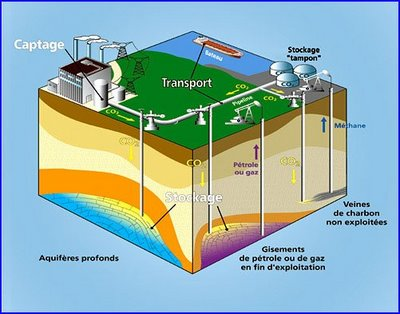
\includegraphics[width=0.75\textwidth]{stockage.jpg}\cite{imstock}
\end{minipage}
\hspace*{\stretch{1}}
\begin{minipage}{0.5\textwidth}
La solution consiste à capturer le \ce{CO2} en le séparant des autres produits auxquels il est lié. Par après, le \ce{CO2} est compressé et convoyé vers l'endroit où il sera stocké et où il ne contribuera plus au réchauffement climatique.
\end{minipage}
 
 

Il existe trois sortes de sites de stockage :
\begin{enumerate}
\item \emph{Réservoirs de pétrole ou de gaz naturel épuisés} Ces réservoirs, qui sont des gisements naturels, ont déjà été utilisés par le passé pour l'extraction du pétrole ou du gaz qui y a séjourné, et on peut donc profiter des installations déjà existantes, comme des canalisations et des puits, pour y injecter le \ce{CO2}. Cela permet de réduire le coût d'enfouissement.

En outre, on sait déjà que ces réservoirs peuvent contenir des hydrocarbures pendant plusieurs millions d'années.

Malheureusement, ces sites ne constituent pas un volume de stockage potentiel extrêmement important.

\item \emph{Aquifères salins\cite{aquisalin}} Ce sont des formations géologiques poreuses qui contiennent de l'eau salée. Cette eau est impropre à la consommation et n'a donc aucun intérêt pour la production d'eau douce. Ils peuvent être situés à terre comme en mer.

Ces réservoirs sont très répandus de par le monde, et constituent un volume potentiel très important. C'est donc un double avantage : le transport sera réduit, et les quantités de \ce{CO2} stockées pourront être conséquentes.

Mais la technologie de stockage dans ces aquifères est encore à approfondir.

\item \emph{Veines de charbon} Dans ce troisième site de stockage, le \ce{CO2} serait absorbé par le charbon, ce qui permettrait à la fois de stocker le dioxyde de carbone et de récupérer du méthane. En effet, les veines de charbon contiennent une grande quantité de gaz, dont du méthane, qui est contenu à l'intérieur de celles-ci. Par adsorption, les molécules de \ce{CO2} se fixent à la surface du charbon, et celui-ci ayant une grande affinité avec le dioxyde de carbone, il relâchera le méthane pour adsorber le \ce{CO2}. Cette technique est appellée "récupération assistée de méthane".

Cette technologie est donc extrêmement prometteuse puisque, non seulement les veines de charbon sont réparties sur l'ensemble de la surface du globe, réduisant ainsi le coût du transport, mais en plus elles permettent également de compenser les coûts d'injection grâce à la réutilisation du méthane pour produire notre ammoniac ! Elle nous permettrait donc de se débarasser du \ce{CO2} tout en nous fournissant du méthane nécessaire à la production de notre ammoniac !

Mais, tout comme pour les aquifères salins, cette technologie est encore à étudier et approfondir. 
 
\end{enumerate}

Le risque de fuites du \ce{CO2} stocké est extrêmement faible : selon un rapport du GIEC (Groupe d'Experts Intergouvernemental sur l'Evolution du Climat), il est très probable que la proportion de \ce{CO2} retenue dans le sol soit encore de plus de 99\% après 1000 ans.

\section{Valorisation}
Le \ce{CO2} peut être injecté dans un puits de pétrole pour chasser les hydrocarbures qui y sont présents. Par exemple, il peut "pousser" le \ce{CH4} et le pétrole pour faciliter leur extraction.

Ainsi, associer le stockage du \ce{CO2} avec la récupération assistée de pétrole ou de méthane pourrait augmenter les bénéfices de l'usine en apportant des revenus provenant de la récupération de ces hydrocarbures.

\begin{figure}[h!]
\caption{Stockage du $CO_2$ \protect \footnotemark}
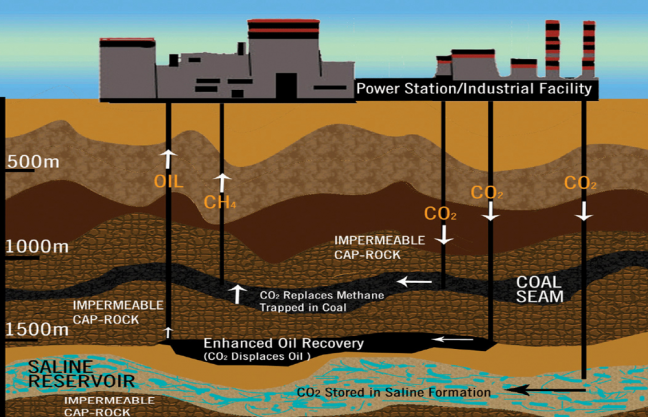
\includegraphics[width=\textwidth]{captureee.png}
\end{figure}
\footnotetext{http://www.wri.org/resources/charts-graphs/carbon-capture-sequestration-flow-chart}


\section{Inconvénients}

Néanmoins, cette solution n'est applicable qu'à certains endroits précis qui doivent réunir plusieurs conditions spécifiques. 

Premièrement, il faut pouvoir atteindre une profondeur suffisante pour permettre au \ce{CO2} d'atteindre un état quasi liquide, ce qui lui fait occuper un volume beaucoup plus faible qu'à l'état gazeux.

Bien que les capacités de stockage de nombreux pays soient encore en cours d'inventaire, le GIEC a estimé les capacités de stockage du \ce{CO2} du monde entier entre 1000 et 10 000 milliards de tonnes. En sachant que notre usine produirait quotidiennement un peu plus de 1200 tonnes de \ce{CO2} par jour, on s'aperçoit alors que cette solution n'est pas encore la solution idéale. Le mieux serait d'associer cette solution à une autre, par exemple une de celles énoncées dans la tâche 3.
 

Il faut également compresser le \ce{CO2}, le transporter jusqu'à l'endroit de stockage puis finalement l'injecter. Il faut en outre creuser les cavités dans lesquelles le \ce{CO2} sera stocké. Tout ceci représente un coût non négligeable.

\section{Impact quantitatif}
Il est assez compliqué de calculer quantitativement l'impact de la solution. Cela dépend de nombreux paramètres, dont le principal est la géo-localisation de l'usine : celle-ci déterminera le coût du transport et de l'injection, la possiblité d'une association du stockage du \ce{CO2} avec la récupération de pétrole ou de méthane, etc.
 

Dans un cadre idéal, si nous arrivions à stocker tout le \ce{CO2} émis, nous éviterions ainsi de rejeter, chaque jour, pour une production quotidienne de 1000 tonnes de \ce{NH3}, 1296 tonnes de \ce{CO2} !


Il ne faut bien sûr pas oublier le coût énergétique que constitue le transport et l'injection du \ce{CO2}.
 

A titre d'indication, le GIEC estimait en 2005 qu'une centrale électrique à cycle mixte de gaz naturel équipée d'un système de captage-stockage de \ce{CO2} aurait besoin de 11\% à 22\% d'énergie de plus qu'une centrale de rendement équivalent non équipée d'un tel système. Si le stockage est sécurisé, et on peut donc supposer que c'est le cas selon le même rapport du GIEC, ce système réduirait les émissions de \ce{CO2} d'environ 80 à 90\%.


\section{Localisation}
Finalement, pour toutes les raisons explicitées dans ce rapport, et compte tenu que notre usine voudrait s'implanter en Europe, nous avons sélectionné plusieurs pays dans lesquels notre usine serait la plus productive et la plus écologique : la Norvège, les Pays-Bas ou encore la Pologne présentent de bons atouts :
\begin{enumerate}
\item Des opérations de stockage du \ce{CO2} ont déjà été entreprises avec succès dans ces pays.
\item Ils présentent de bons sites de stockage tels qu'énoncés et détaillés ci-avant.
\item Le méthane, nécessaire pour les réactions des reformages primaire et secondaire ainsi que pour le four, y est naturellement présent en grande quantité.
\end{enumerate}

\printbibliography[heading=bibintoc]

\end{document}
